% manuscript.tex
% Purpose: assemble the report. This file writes NO numbers itself; it
% \input{}s the LaTeX table fragments Stata exported and \includegraphics{}s
% the PDF figures R exported. Compile this from inside the report/ folder
% (the ../output/... paths below assume that working directory).
% A comment sits above every line explaining what that line does.

% Use the standard "article" class at 11pt base font size.
\documentclass[11pt]{article}
% Set all page margins to 0.85 inch so text isn't cramped.
\usepackage[margin=0.85in]{geometry}
% Load booktabs for the clean horizontal rules esttab's tables use.
\usepackage{booktabs}
% Load graphicx so we can \includegraphics the figure PDFs.
\usepackage{graphicx}
% Load amsmath for nicely typeset equations.
\usepackage{amsmath}
% Load caption so we can style figure/table captions consistently.
\usepackage{caption}
% Use proper T1 font encoding so accented/special characters render well.
\usepackage[T1]{fontenc}
% Use Latin Modern fonts, a clean modern look for the default font family.
\usepackage{lmodern}
% Remove the automatic paragraph-first-line indent.
\setlength{\parindent}{0pt}
% Add a little vertical space between paragraphs instead.
\setlength{\parskip}{6pt}
% Make captions small and bold-label ("Table 1", "Figure 1") for readability.
\captionsetup{font=small,labelfont=bf}
% Reserve one reusable "box" to measure a table's width, so its notes
% paragraph below can be set to that same width (see the DiD table).
\newsavebox{\tablebox}

% Set the document title.
\title{Two Empirical Designs with Synthetic Court Data}
% Set the author name.
\author{Shamayla Durrin Islam}
% Set the date shown under the title.
\date{September 2026}

% Begin the actual document content.
\begin{document}
% Typeset the title, author, and date block defined above.
\maketitle

% State the report's purpose plainly, including that the data is fictional.
\textbf{Purpose.} This report presents a difference-in-differences
estimation and a regression discontinuity estimation on two fictional
datasets constructed for this exercise. Each dataset has a treatment effect
purposely built into it; the goal is to recover that effect and to present
the resulting estimates, tables, and figures clearly. All data, districts,
and cases are fictional; results are a demonstration of estimation and
reporting practice, not evidence about real courts.

% Start an unnumbered section describing the data.
\section*{Data}

% Subsection for the district-level DiD dataset.
\textbf{Court district data.} We construct 40 fictional court districts.
In 2019, 20 of them adopt a reform meant to speed up case processing; the
other 20 never do. We observe all 40 districts every year from 2015 through
2022, tracking one outcome: the average number of days it takes to process
a case in that district that year.

% Subsection for the case-level RD dataset.
\textbf{Fast-track case data.} We separately construct 1,000 individual
court cases, each assigned a continuous priority score between 30 and 70.
Cases scoring 50 or above are eligible for a fast-track program. The
outcome is the number of days it takes to process that case.

% Start an unnumbered section for the summary-statistics table.
\section*{Summary statistics}

% Start a centered block to hold the two-panel summary-statistics table.
\begin{center}
% Give this table a caption/number via the caption package's captionof.
\captionof{table}{Descriptive statistics}
% Panel label for the district-year variables, then break the line.
\textit{Panel A. District-year panel, 2015--2022}\\[2pt]
% Insert the LaTeX fragment esttab wrote for Panel A, then break the line
% and add space before the next panel (without this "\\", the following
% label would run onto the same line as the table instead of below it).
{
\def\sym#1{\ifmmode^{#1}\else\(^{#1}\)\fi}
\begin{tabular}{l*{1}{ccccc}}
\toprule
                    &           N&        Mean&          SD&         Min&         Max\\
\midrule
Case-processing delay (days)&         303&       54.15&        4.76&       41.75&       67.52\\
Reform district     &         320&        0.50&        0.50&        0.00&        1.00\\
\bottomrule
\end{tabular}
}
\\[8pt]
% Panel label for the case-level variables, then break the line.
\textit{Panel B. Individual cases, full sample}\\[2pt]
% Insert the LaTeX fragment esttab wrote for Panel B.
{
\def\sym#1{\ifmmode^{#1}\else\(^{#1}\)\fi}
\begin{tabular}{l*{1}{ccccc}}
\toprule
                    &           N&        Mean&          SD&         Min&         Max\\
\midrule
Case-processing duration (days)&         940&       57.35&        8.36&       30.37&       81.60\\
Priority score      &        1000&       50.02&       11.90&       30.03&       69.88\\
Eligible for fast-track processing&        1000&        0.51&        0.50&        0.00&        1.00\\
\bottomrule
\end{tabular}
}

% End the centered block.
\end{center}
% Add small-font notes explaining exactly what the table's numbers mean.
{\footnotesize Notes: Panel A summarizes district-year observations for
40 districts from 2015 through 2022; 20 districts adopt the fictional
reform in 2019. Panel B summarizes individual cases over the full
priority-score range. Fast-track eligibility equals one for scores of at
least 50. Statistics are unweighted and calculated using nonmissing
observations for each variable.}

% Start an unnumbered section for the DiD design.
\section*{Difference-in-differences}

% Start a centered block to hold the DiD trends figure (shown first,
% before any equation or table, since the text below discusses it first).
\begin{center}
% Include the DiD figure PDF that R produced, sized to 72% of text width.
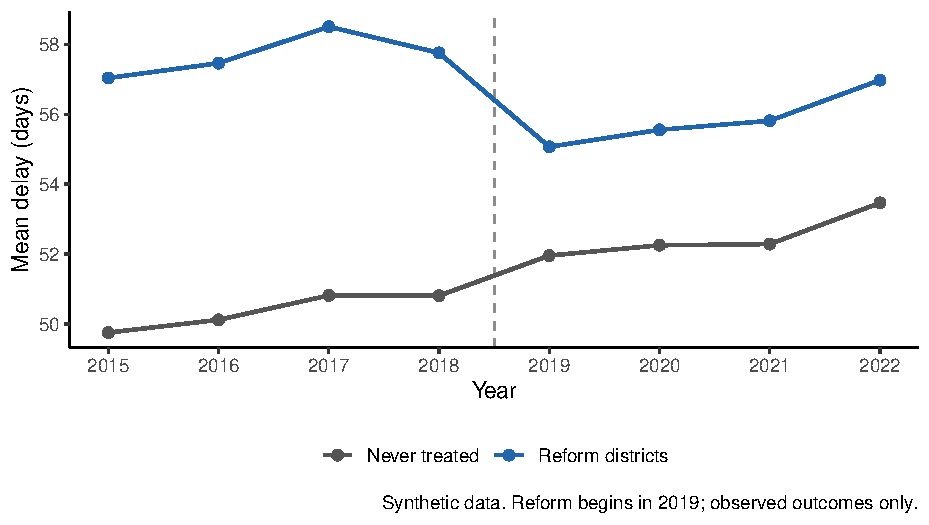
\includegraphics[width=0.72\linewidth]{../output/figures/did.pdf}
% Caption/number this figure.
\captionof{figure}{Observed mean delay by treatment group}
% End the centered block.
\end{center}

% Discuss the visual pattern in Figure 1 and the identifying assumption.
Figure 1 shows broadly similar pre-reform movements, although reform
districts experience a decline in 2018 that is not mirrored by the
comparison group. This visual evidence is informative but cannot
establish parallel untreated trends. In this simulation, that assumption
holds in expectation because both groups share a common untreated trend
and mean-zero shocks.

% Transition from the visual evidence to the formal regression, then
% show the equation right before the table it describes.
We estimate a model with district and year fixed effects, identifying
the reform effect from the differential change after adoption. Standard
errors are clustered by district to account for dependence across years.
The model specification is given below:
% Show the DiD model equation.
\[
Y_{jt}=\alpha_j+\lambda_t+\tau(Treated_j\times Post_t)+u_{jt}.
\]

% Start a centered block to hold the DiD regression table.
\begin{center}
% Caption/number this table.
\captionof{table}{District reform and processing delay}
% Measure the table's width into \tablebox, then draw it, so the notes
% paragraph below can be set to that exact same width. Using "\global" is
% essential here: a plain \sbox only assigns within the current group, and
% \begin{center}...\end{center} is itself a group, so without "\global"
% \tablebox would revert to empty (zero width) as soon as this center block
% closes, breaking the notes' width below.
\global\sbox{\tablebox}{{
\def\sym#1{\ifmmode^{#1}\else\(^{#1}\)\fi}
\begin{tabular}{lc}
\toprule
 & (1)\\
Dependent variable: & Delay (days)\\
\midrule
Reform district $\times$ Post-reform&      -4.197\sym{***}\\
            &     (0.639)         \\
\midrule
District fixed effects&         Yes         \\
Year fixed effects&         Yes         \\
Observations&         303         \\
District clusters&          40         \\
\bottomrule
\end{tabular}
}
}
\usebox{\tablebox}\\[6pt]
% Add notes sized to the table's own width (matching \tablebox), rather
% than the full page width, as in standard published regression tables.
% (Kept in the same center block as the table above, rather than a
% second \begin{center}...\end{center}, to avoid stacking two sets of
% that environment's own extra spacing on top of each other.)
\begin{minipage}{\wd\tablebox}
{\footnotesize Notes: OLS with district and year fixed effects, estimated
by \texttt{regress}. Standard errors, clustered by district, are shown in
parentheses below the coefficient. * p$<$0.10, ** p$<$0.05, *** p$<$0.01.
Observations exclude missing outcomes.}
\end{minipage}
% End the centered block.
\end{center}

The estimated reform effect is $-4.197$ days (95\% CI $[-5.490,-2.904]$),
close to and statistically indistinguishable from the built-in simulated
effect of $-4$ days, as expected in this fully specified synthetic design.

% Start an unnumbered section for the RD design.
\section*{Regression discontinuity}

% Introduce the eligibility rule and why a naive comparison would confound
% eligibility with the score itself.
Fast-track eligibility is determined by whether a case's priority score
reaches 50. Because processing duration also varies with the score,
comparing all eligible and ineligible cases would confound eligibility
with systematic score differences. We instead compare cases near the
cutoff, allowing the score--duration relationship to differ on either side.

% Start a centered block to hold the RD figure (shown first, before any
% equation or table, since the text below discusses it first).
\begin{center}
% Include the RD figure PDF that R produced, matching the DiD figure's
% width exactly for visual consistency.
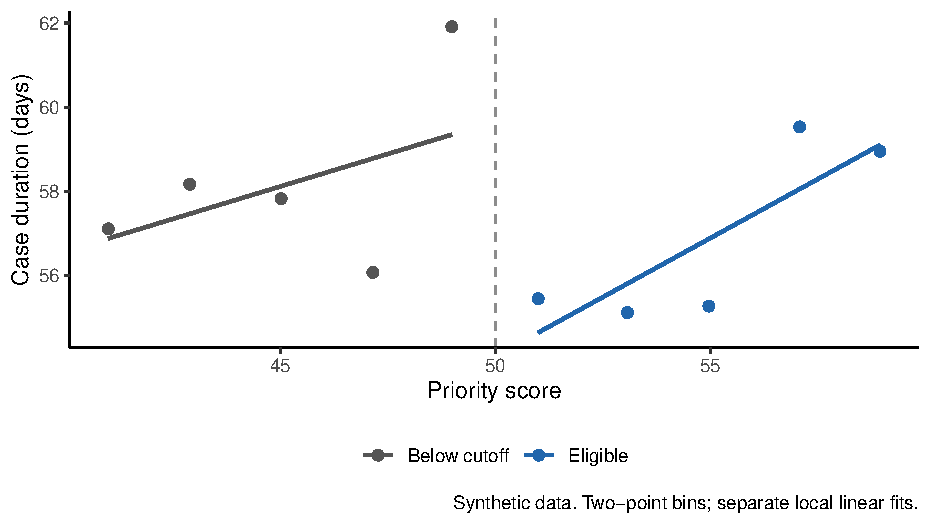
\includegraphics[width=0.72\linewidth]{../output/figures/rd.pdf}
% Caption/number this figure.
\captionof{figure}{Binned outcomes around the eligibility cutoff}
% End the centered block.
\end{center}

% Discuss the visual pattern in Figure 2 and the identifying assumption.
Figure 2 displays binned outcome means and separate fitted relationships
around the threshold. The downward discontinuity motivates estimating a
local treatment effect, but the outcome plot alone cannot establish the
design's validity. Identification requires potential outcomes to vary
continuously at 50, without precise sorting or another intervention
changing at the same threshold.

% Define the centered score and eligibility indicator, then show the
% equation right before the table it describes.
With $x_i=Score_i-50$ and $D_i=1\{Score_i\ge50\}$:
% Show the RD model equation.
\[
Y_i=a+\tau D_i+b x_i+dD_ix_i+e_i,\qquad |x_i|\le10.
\]

% Start a centered block to hold the RD regression table.
\begin{center}
% Caption/number this table.
\captionof{table}{Fast-track eligibility and case duration}
% Measure the table's width into \tablebox (globally, so it survives past
% this center block), then draw it, so the notes below match its width.
\global\sbox{\tablebox}{{
\def\sym#1{\ifmmode^{#1}\else\(^{#1}\)\fi}
\begin{tabular}{lc}
\toprule
 & (1)\\
Dependent variable: & Duration (days)\\
\midrule
Fast-track eligibility&      -5.574\sym{***}\\
            &     (1.481)         \\
\midrule
Bandwidth   &          10         \\
Polynomial order&Local linear         \\
Separate slopes across cutoff&         Yes         \\
Observations&         457         \\
\bottomrule
\end{tabular}
}
}
\usebox{\tablebox}\\[6pt]
% Add notes sized to the table's own width, matching the DiD table's
% style (kept in the same center block as the table, not a second one).
\begin{minipage}{\wd\tablebox}
{\footnotesize Notes: Individual-level local linear OLS with separate
slopes on either side of the cutoff, uniform weights, and a fixed
bandwidth of 10 score points. Heteroskedasticity-robust standard error
shown in parentheses below the coefficient. * p$<$0.10, ** p$<$0.05,
*** p$<$0.01. This is not bias-corrected RD inference.}
\end{minipage}
% End the centered block.
\end{center}

Within the 10-point bandwidth, fast-track eligibility reduces estimated
processing duration by 5.57 days (95\% CI: $-8.48$ to $-2.66$); this is a
local estimate at the cutoff.

% Close with a short, honest limitations paragraph.
\textbf{Limitations.} Identification is built into the simulation.
Real policy research would require investigating assignment, missingness,
measurement, spillovers, and specification sensitivity. The RD bandwidth
is chosen for this demonstration, not selected from real evidence.
% End the document.
\end{document}
